\section{Vector Field Visualization} % (fold)
\label{sec:vector_fields}
%
A vector field $\vv(\vx,t): D \times T \mapsto \RRSet^n$ is a map from spatial
and temporal domains $D \subset \EESet^n$ and $T \subset \RRSet$ to the
$n$-dimensional vector space $\RRSet^n$.
%
Just like a scalar field, it assigns a value to each position and time in the
domains, but this time the value is a vector.
%
Examples for vector fields are the velocity of a fluid flow, the displacement
field of a deformed object, and the magnetic field around an electromagnet.
%
If the vector field does not change with time, or we are only interested in the
field at a single instant, we say that we have a \emph{steady} vector field
$\vv(\vx)$.
%
If the vector field changes with time, we call it an \emph{unsteady} vector
field.
%
If we are talking about a vector field representing the velocity of a fluid
flow, we sometimes call it a (steady or unsteady) \emph{flow field}.
%

%
Vector field visualization methods can be sorted into roughly six different
classes: Basic methods, image-based methods, integral curves and -surfaces,
topological features, vortex extraction and \acl{LCS}.
%
We will again visit the most important methods in the following sections.
%

%
\subsection{Basic Methods} % (fold)
\label{sub:vector_basic}
%
Basic methods display the vector data using simple techniques, much like
image-based methods for scalar fields.
%
They encompass techniques such as \emph{arrow plots}, or \emph{color-mapping}
the velocity magnitude, vorticity and other derived quantities directly.
%

%
\subsubsection{Arrow Plots}
%
Arrow plots are the simplest way to visualize a vector field.
%
In such a plot, arrow glyphs are placed at multiple locations throughout the
domain.
%
The arrows are aligned with the direction of the local vector, and their
length is typically scaled based on its magnitude.
%
Such plots can very accurately show the vectors at a limited number of
locations, but they quickly become cluttered once too many arrows are plotted,
or the arrows become too long and occlude each other.
%

%
\subsubsection{Color-Mapping}
%
Color-mapping can be applied to vector fields in different ways.
%
The most common one is simply displaying the magnitude of the vector field as a
scalar.
%
Other scalars derived from the vector field, such as the vorticity magnitude and
divergence, can be visualized in the same way.
%
All of this obviously goes along with a loss of information.
%
Since color has three degrees of freedom, a vector field can also be visualized
without information loss by directly mapping the vector values to colors.
%
The most naive way is to simply interpret the three components of a \ac{3D}
vector as RGB values.
%
Such images theoretically contain they full information of the original vector
field.
%
However, they are very hard to interpret, as there is no inherent meaningful
connection between the direction of the vector and the color it is mapped to.
%
This can be slightly improved for \ac{2D} vector fields by mapping the angle
and magnitude of the vector to hue and value of the HSV color space.
%
% subsection direct_methods (end)
%
\subsection{Image-Based Methods} % (fold)
\label{sub:vector_image_based}
%
Image-based methods visualize the vector data by generating a space-filling
texture.
%
Among such methods are \emph{line integral convolution}, \emph{spot noise},
and \emph{texture advection}.
%

%
\subsubsection{Line Integral Convolution}
%
Line integral convolution (\acs{LIC}\acused{LIC})\cite{Cabral1993} is the most
popular image-based vector field visualization method.
%
It is based on ``smearing'' a random noise texture along stream lines of a
\ac{2D} vector field.
%
More specifically, the color at a certain position is determined as a weighted
integral of the color values encountered along a stream line passing through
that position.
%
The result is a space-filling image where the direction of the vector field is
visible at each location (see \cref{fig:lic_topo}).
%
The basic \ac{LIC} technique is only applicable to \ac{2D} steady vector fields,
but extensions have been developed for \ac{3D}~\cite{Rezk-Salama1999} and
unsteady~\cite{Shen1997} datasets.
%

%
\subsubsection{Spot Noise}
%
Spot noise is also a method designed for \ac{2D} data and produces results
similar to \ac{LIC}~\cite{Wijk1991,Leeuw1995}.
%
It works by blending noise sprites that have been stretched and rotated
according to the local vector direction.
%
In contrast to \ac{LIC}, spot noise better represents the local vector
magnitude, but in regions with low magnitude, the vector direction is not well
visible.
%

%
\subsubsection{Texture Advection}
%
Texture advection works on \ac{2D} steady and unsteady vector fields.
%
It is best suited for vector fields representing a flow, as it simulates the
transport(advection) of a texture with the flow.
%
A texture is placed in the flow at some point in time, and each point on the
texture is moved with the flow over time.
%
As time progresses, the texture is warped, and the viewer can follow where each
part of the texture is transported.
%
This method has a lot in common with the integration-based methods presented in
the next section.
%
In fact, texture advection simply displays a time surface with a mapped texture
in a \ac{2D} vector field.
%

%
% subsection vector_image_based (end)
%
\subsection{Integral Curves and -Surfaces} % (fold)
\label{sub:integral_curves_and_surfaces}
%
Integral curves and -surfaces are generated by integrating the vector field
starting from different kinds of seed structures.
%
Depending on the seeding strategy and the kind of vector field, we can obtain
\emph{streamlines}, \emph{pathlines}, \emph{streaklines}, \emph{timelines},
and the accompanying surfaces\ToCite{Batchelor}.
%
Since integral structures play an important role in several parts of this
thesis, we will cover them here in more detail.
%
\begin{figure}[t]
    \centering
    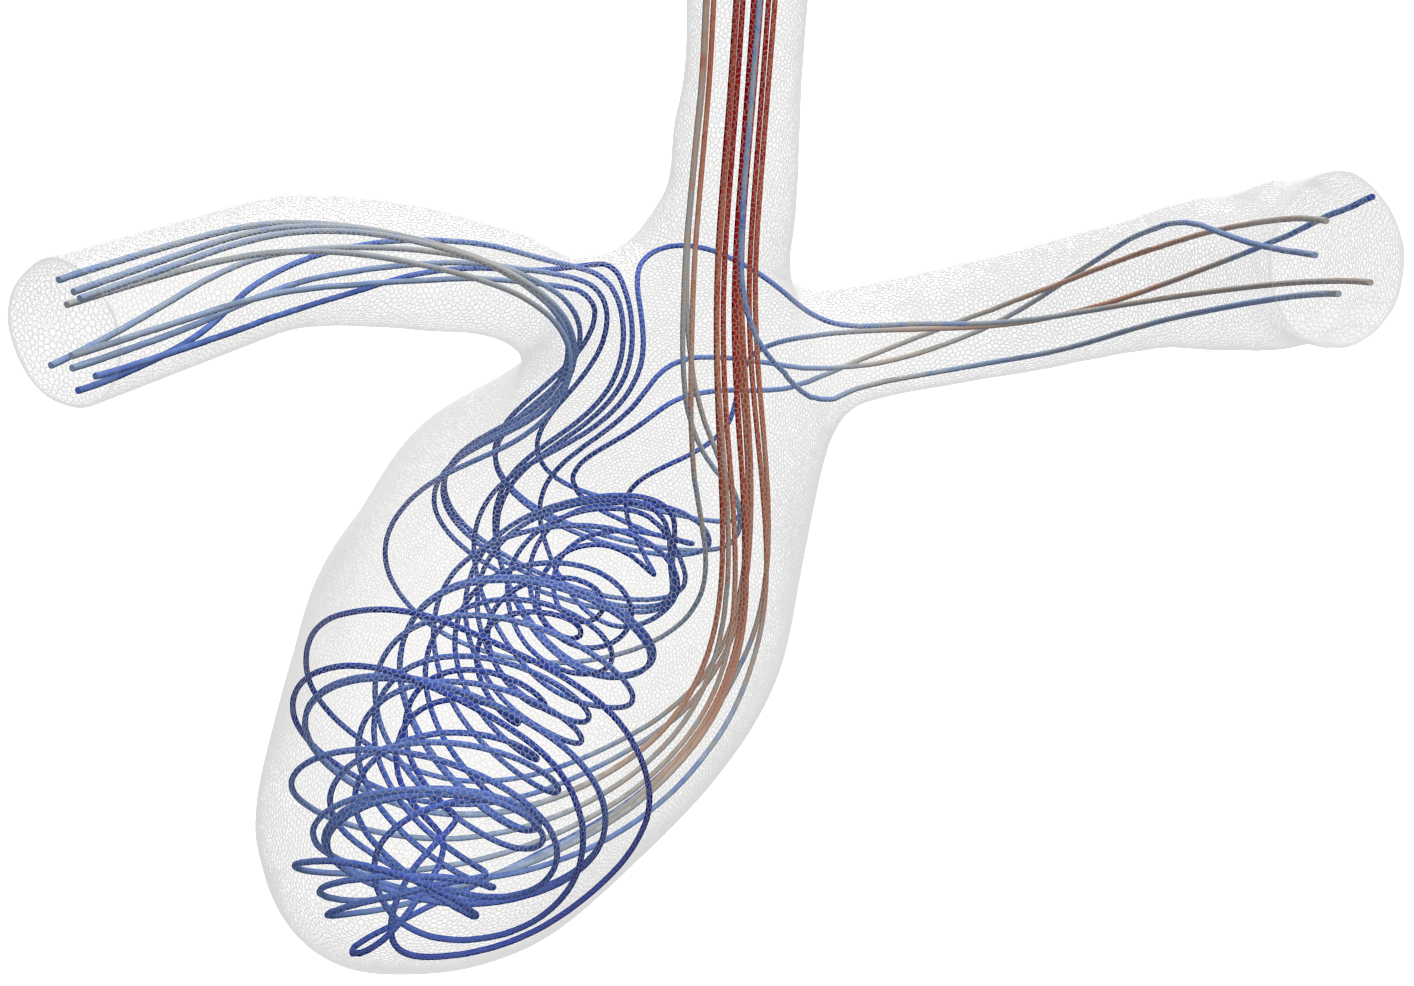
\includegraphics[width=0.9\textwidth]{figures/pathlines_aneurysm.png}
    \caption{Streamlines in the simulated flow through a cranial aneurysm.
             Image courtesy of Tim Gerrits~\cite{Gerrits2018}.}
    \label{fig:streamlines}
\end{figure}
%

\subsubsection{Streamlines} % (fold)
\label{ssub:streamlines}
%
Streamlines are the simplest form of integral curve in a vector field.
%
They are defined for steady vector fields.
%
Depending on the application area, they are also sometimes called \emph{field
lines}.
%
A streamline is a curve that is tangent to the vector field everywhere along its
path.
%
Given a streamline $\vc(s)$ of the steady vector field $\vv(\vx)$, this means
that $\vc(s) \times \vv(\vc(s))$ is $\vNull$ for all $s$.
%
This criterion is valid for any parameterization of the curve, but we can only
use it to check if a given curve is a streamline.
%
To compute streamlines, we typically solve the ordinary differential equation
%
\begin{equation*}
    \frac{\partial \vc(s)}{\partial s} = \vv(\vc(s))
    \text{, with } \vc(0) = \vx_0 \, \text{.}
\end{equation*}
%
This yields a streamline with a particular parameterization: an integral curve
of the vector field.
%
Due to their definition, two stream lines never intersect at single points.
%
They are either completely disjoint, or they coincide.
%

%
Visualizing a steady vector field with stream lines shows the direction of the
flow much like a \ac{LIC} image does, but not in a space-filling manner.
%
This allows for use of streamlines also in \ac{3D} data (see
\cref{fig:streamlines}).
%
Streamline visualization can be deceiving when used on single time slices of
an unsteady flow field.
%
The connected lines mistakenly suggest paths of fluid elements.
%
However, if the flow field changes significantly with time, the actual paths of
fluid elements can deviate significantly from the streamlines in a single time
slice.
%
In this case, the more appropriate visualization tools are pathlines,
streaklines, and timelines, which incorporate the temporal information of the
flow.
%
% subsubsection streamlines (end)

\subsubsection{Pathlines} % (fold)
\label{ssub:pathlines}
%
Pathlines describe the paths of massless particles moving with a
flow.
%
They are defined as the solution to the ordinary differential equation
%
\begin{equation*}
    \frac{\partial \vc(t)}{\partial t} = \vv(\vc(t), t)
    \text{, with } \vc(t_0) = \vx_0 \, \text{,}
\end{equation*}
%
where $\vc(t)$ is the curve of the pathline, $t$ is time, and $\vv(\vx, t)$ is
an unsteady vector field.
%
Looking at this definition, it becomes apparent that for a steady vector field,
which does not change with time, streamlines and pathlines are identical.
%

%
The set of all pathlines for all possible combinations of start position
$\vx$, start time $t_0$ and end time $t$ forms the \emph{flow map}.
%
This function, which we write as $\bPhi(\vx, t_0, t)$, determines where a
massless particle starting at position $\vx$ and time $t_0$ ends up after
advecting with the flow until time $t$.
%

%
Pathlines allow the visualization of the dynamic behavior of an unsteady flow
in a static image.
%
To show the temporal information, the time is often color-mapped on the curve.
%
Unlike streamlines, pathlines can and do intersect each other.
%
For very complex flows, showing a lot of pathlines can therefore quickly become
confusing.
%
In such cases it can be better to show animated streaklines instead.
%
% subsubsection pathlines (end)

\subsubsection{Streaklines} % (fold)
\label{ssub:streaklines}
%
Streaklines are the connected locations of a continuously injected
stream of massless particles into a flow.
%
They approximate the behavior of a thin stream of dye injected at a certain
position that is often applied in experimental settings to visualize the flow.
%
Formally, a streakline is formed by the connected endpoints of a set of
pathlines with the same start position and end time, but continuously increasing
start time.
%
Using the flow map $\bPhi$, which we introduced earlier, we can formally define
a streakline as
%
\begin{equation*}
    \vc(s) = \bPhi(\vx, s, t)\,\text{,}
\end{equation*}
%
where $t$ is the current time, $\vx$ is the injection point, and $s$ is the
continuously increasing start time that runs along the curve.
%
Like pathlines, streaklines also become identical to streamlines if the flow
does not change with time.
%

%
While a pathline shows the behavior of the flow over a period of time, a
streakline only ever shows the position of the injected particles at a
single time instant.
%
Streaklines are therefore often animated by continuously increasing the end
time $t$ and injecting more particles.
%
This again mirrors the behavior of injected dye observed in an experiment.
%
% subsubsection streaklines (end)

\subsubsection{Timelines} % (fold)
\label{ssub:timelines}
%
Timelines are different from all the previous integral lines in that
their seeding structure is not a single point, but a whole line.
%
A timeline is formed by placing a line somewhere in the flow, treating it as a
set of massless particles, and letting the whole line advect with the flow at
once.
%
Formally, a time line is formed by the connected endpoints of a set of pathlines
with the same start and end time, but continuously changing start position.
%
Given a seed curve $\vs(s)$ and start and end times $t_0$ and $t$, we can
formally define a timeline in terms of the flow map as
%
\begin{equation*}
    \vc(s) = \bPhi(\vs(s), t_0, t)\,\text{.}
\end{equation*}
%
Much like streaklines, timelines are often animated to show the progressive
effect of the flow.
%
As the end time $t$ advances, the line is transported and warped by the flow and
visualizes the way the flow mixes and perturbs a region of the fluid.
%
\begin{figure}[t]
    \centering
    \MissingFigure{Image illustrating relationship between pathlines,
    streaklines and timelines}
    \caption{Pathlines, streaklines and timelines of a \ac{2D} vector field.}
    \label{fig:path_streak_timelines}
\end{figure}
%
% subsubsection timelines (end)

\subsubsection{Integral Surfaces} % (fold)
\label{ssub:integral_surfaces}
%
Integral surfaces can be formed from any of the integral lines by using a
higher-dimensional seeding structure.
%
For stream-, path-, and streaklines this means using a line as the seeding
structure.
%
Timesurfaces are formed by using a surface as the seed.
%
Integral surfaces can be helpful for visualization because they have a better
visual coherency than a number of single lines.
%
The curvature, wrinkling and folding of structures induced by the flow become
easier to grasp when using integral surfaces.
%
On the flip side, integral surfaces have more of a problem with occlusion
compared to lines, as they are more massive.
%
% subsubsection integral_surfaces (end)

%
% subsection integral_lines_and_surfaces (end)
%
\subsection{Vector Field Topology} % (fold)
\label{sub:vector_field_topology}
%
% The topology of a vector field is defined by \emph{critical points},
% \emph{boundary switch points/lines}, \emph{attachment- and detachment
% points/lines}, the accompanying \emph{separatrices} connecting these points,
% and \emph{isolated closed streamlines}.
%
The topology of a vector field is defined by \emph{critical points},
\emph{separation- and attachment points} and the accompanying
\emph{separatrices} connecting them.
%
Together, they form a sort of skeleton of the vector field, from which the
behavior of the full field can be inferred.
%
\begin{figure}[t]
    % \centering
    \begin{captionbeside}
        {\ac{LIC} of a \ac{2D} vector field with overlaid vector field topology
        consisting of critical points, boundary switch points, and separatrices.
        Image source: Tino Weinkauf~\cite{Weinkauf2008}.\label{fig:lic_topo}}
        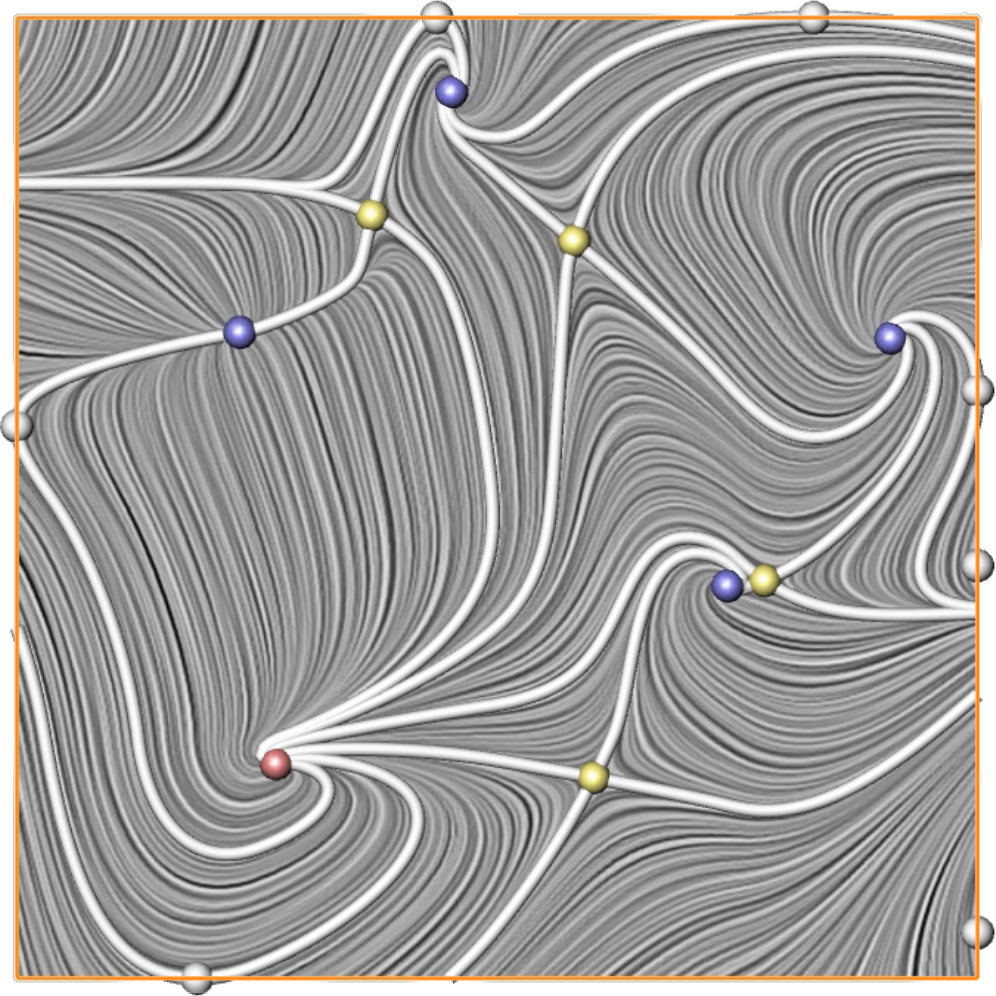
\includegraphics[width=0.6\textwidth]{figures/lic_topology.png}
    \end{captionbeside}
\end{figure}
%

\subsubsection{Critical Points} % (fold)
\label{ssub:critical_points}
%
Critical points of a vector field are locations where the magnitude
of the vector becomes zero.
%
They are interesting because they are at the centers of interesting structures
in the vector field.
%
Critical points in vector fields can be sorted into different categories.
%
Which category a critical point belongs to depends on the behavior of the vector
field in its vicinity, which is encoded in its derivative.
%
The Jacobian matrix $\mJ(\vv) = \vv \T{\nabla}$ gathers the partial derivatives
of all components of the vector field.
%
The signs of the real parts of its eigenvalues indicate if the vector field is
attracting or repelling in the vicinity of the critical point.
%
Depending on these signs, the critical point can be categorized into
\emph{sinks} (negative), \emph{sources} (positive), and \emph{saddles} (mixed
signs).
%
The presence of an imaginary part of the eigenvalues/eigenvectors indicates
swirling behavior.
%
A more in-depth discussion of critical points in vector fields has been provided
by Helman and Hesselink~\cite{Helman1991}.
%
% subsubsection critical_points (end)

%
% \paragraph{Boundary switch points/lines} are locations where the vector field
% is parallel to the boundary of the domain.
% %
% They separate inflow and outflow boundary regions.
% %

\subsubsection{Separation- and Attachment Lines/Surfaces} % (fold)
\label{ssub:separation_attachment_lines}
%
Separation- and attachment lines/surfaces occur on no-slip boundaries.
%
They are locations where the flow separates from/attaches to a surface.
%
In a \ac{2D} flow, these are points.
%
In \ac{3D}, they can be point or line structures.
%
Separation- and attachment structures are similar to critical points of the
vector field, specifically to saddles, in that they are end points of
streamlines of the vector field.
%
However, they are not exactly critical points, as the velocity is zero
everywhere on a no-slip boundary.
%
Instead, they are topological features of the skin friction field, which
describes the shear of the flow near the boundary~\cite{Surana2006}.
%
% subsubsection separation_attachment_lines (end)

\subsubsection{Separatrices} % (fold)
\label{ssub:separatrices}
%
Separatrices connect critical points with each other.
%
They are lines in \ac{2D} vector fields and can be lines or surfaces in \ac{3D}
vector fields~\cite{Helman1989,Helman1991}.
%
Separatrices start at saddle points or separation-/attachment points.
%
They are streamlines with a special property: Streamlines passing through two
points on opposite sides of the separatrix will diverge from each other near a
saddle or separation-/attachment point in forward or backward flow direction.
%
As such, they separate the flow into distinct regions that streamlines starting
in these regions will never leave.
%
Because streamlines and separatrices are an instantaneous observation (they
exist in steady vector fields or at single points in time in an unsteady vector
field), this does not imply that pathlines will never leave these regions in
unsteady flow.
%
For unsteady flows, the equivalent of separatrices are \acl{LCS}, which we will
cover in the next section.
%
% subsubsection separatrices (end)
%
% subsection vector_field_topology (end)
%
\subsection{Vortex Extraction} % (fold)
\label{sub:vortex_extraction}
%
Vortices are structures in a flow that show a swirling motion around a common
center.
%
They will usually stay intact for long periods of time.
%
Vortices are the defining characteristic of turbulent flow.
%
The study of their behavior is a central topic of current fluid dynamics
research.
%
Even though the concept of a vortex seems rather simple, hundreds of years of
fluid dynamics research still has not resulted in a universally accepted formal
definition.
%
This is why there is a plethora of methods for detecting and quantifying
vortices in the literature.
%
Most methods can be sorted into two categories: \emph{region-based} and
\emph{line-based}.
%
They can be further classified by their invariance to transformations of the
reference frame through which the flow is observed.
%
Non-invariant methods are sensitive to all reference frame transformations.
%
Galilean invariant methods are insensitive to any motion of the reference frame
with constant speed and direction.
%
Objective methods are insensitive to any smooth translation and rotation of the
reference frame.
%
We will cover some significant vortex extraction methods here.
%
An extensive survey on the subject has been done by G\"unther and
Theisel~\cite{Guenther2018}.
%

%
Region-based methods measure the ``vortex-ness'' of the flow at a point by a
scalar quantity.
%
Applying a threshold to this quantity shows the vortex regions.
%
Notable representatives of this category are the \emph{vorticity magnitude},
\emph{$\lambda_2$-criterion} and \emph{Q-criterion}, which are all Galilean
invariant methods that work on steady vector fields.
%
Recently, the \emph{\acl{IVD}}~(\acs{IVD}) has been proposed as an objective
criterion for steady vector fields.
%
Its extension, the \emph{\acl{LAVD}}~(\acs{LAVD}) also accounts for unsteady
behavior of the flow.
%
Region-based approaches are generally simple and efficient to implement, but the
results are dependent on the choice of the threshold, and they do not produce
explicit representations of the vortices.
%

%
Line-based methods explicitly extract the vortex core line that is the center
of the swirling behavior.
%
The \emph{reduced velocity} approach for extracting vortex core lines in steady
flows was proposed by Sujudi and Haimes~\cite{Sujudi1995} and later identified
as an application of the \emph{parallel vectors} operator by Peikert and
Roth~\cite{Peikert1999}.
%
This approach is only Galilean invariant when applying it to \ac{2D} vector
fields.
%
A Galilean invariant approach for finding the \emph{cores of swirling particle
motion} in unsteady flows was proposed by Weinkauf \etal \cite{Weinkauf2007}.
%
Recently, G\"unther \etal~\cite{Guenther2017} provided a framework for
objective vortex core detection.
%
This is realized by determining a locally \emph{near-steady frame} for observing
the flow.
%
\begin{figure}[t]
    \centering
    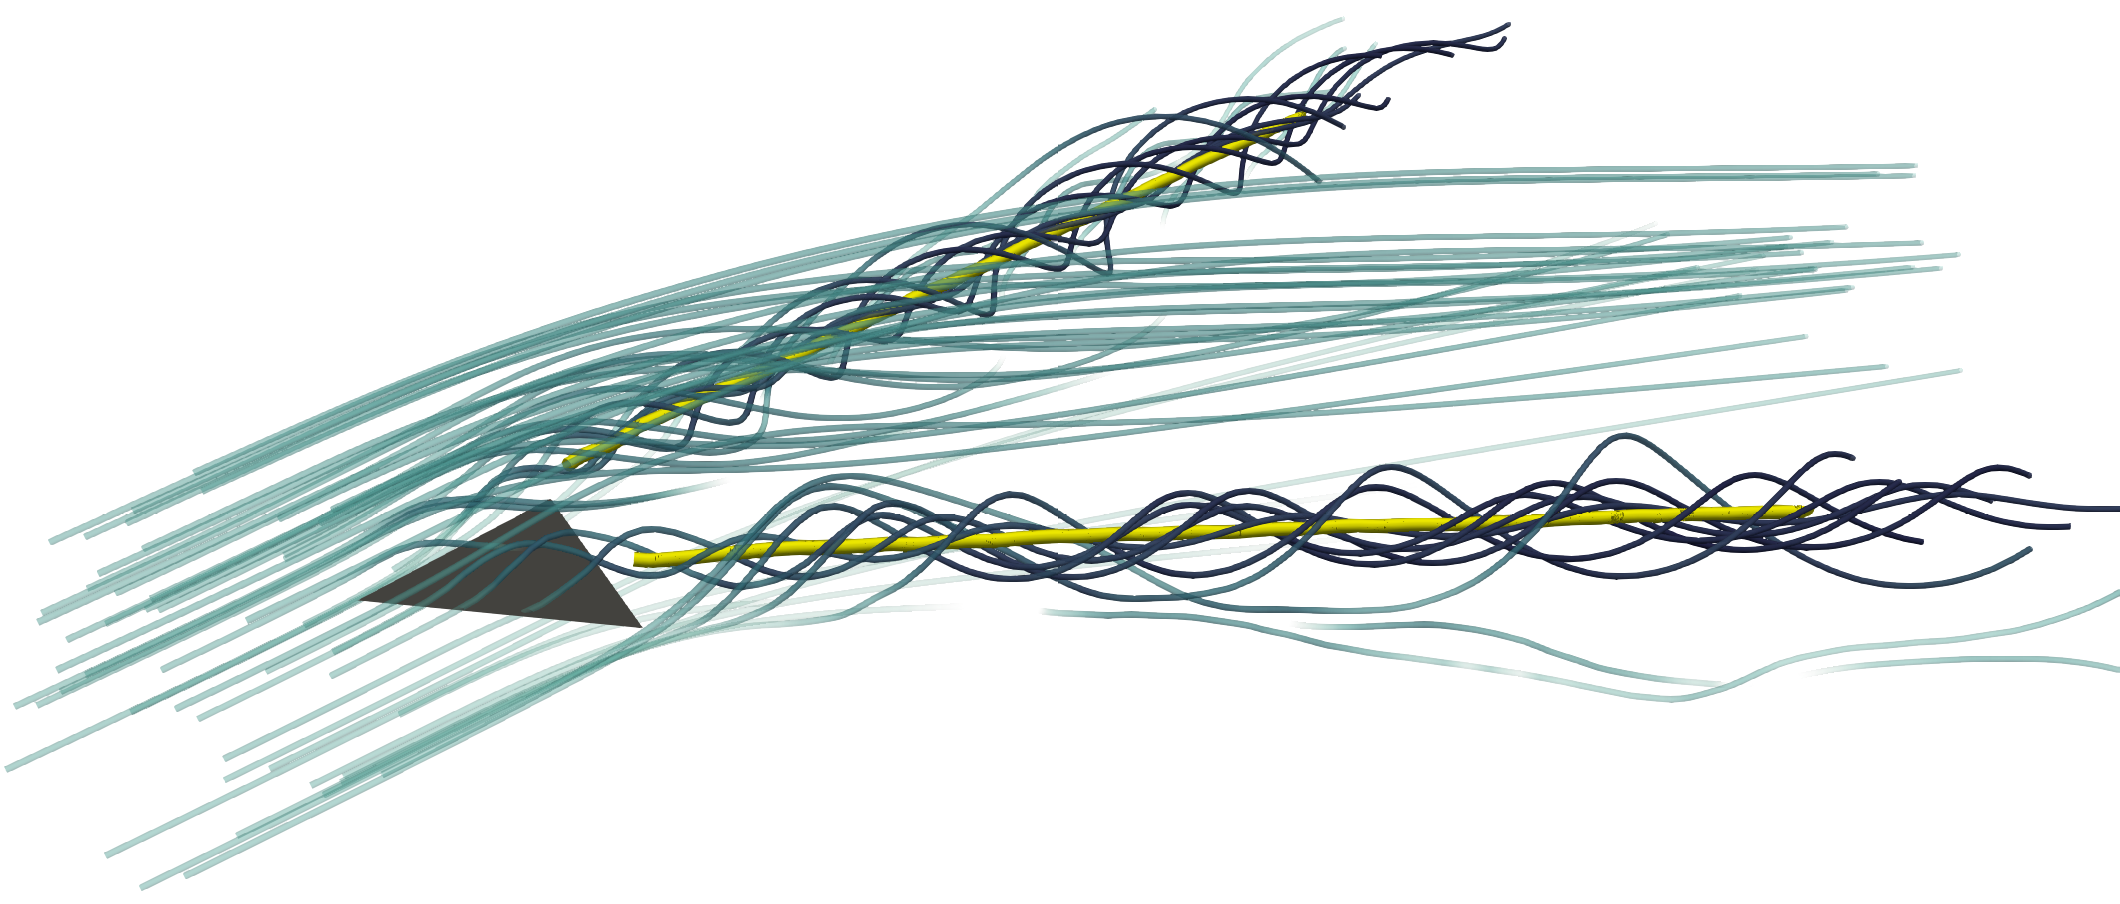
\includegraphics[width=\linewidth]{figures/DeltaWingStreamlines.png}
    \caption{Vortex core lines (yellow) and streamlines (blue) in the steady
    flow around a delta wing.}
    \label{fig:delta_wing_vortex_cores}
\end{figure}
%

%
\subsubsection{Vorticity Magnitude} % (fold)
\label{ssub:vorticity_magnitude}
%
The vorticity is commonly used in fluid dynamics literature to characterize the
rotational behavior of the flow.
%
It is defined as the curl of the flow field $\nabla \times \vv$.
%
The result is a vector field that points in the direction of the local axis of
rotation and whose magnitude indicates the rotation strength.
%
Vorticity magnitude is sometimes used to detect vortices.
%
However, a constant threshold over the whole domain is often not sufficient to
detect and distinguish all vortices, and it might yield false-positives in shear
flow.
%
This is why other methods often perform better.
%
% subsubsection vorticity_magnitude (end)
%
\subsubsection{Q-Criterion} % (fold)
\label{ssub:q_criterion}
%
The Jacobian $\mJ$ of a flow field can be decomposed into a symmetric part $\mS$
(often called \emph{strain rate tensor}) and an asymmetric part $\bOmega$ (often
called \emph{vorticity tensor}) where
%
\begin{equation*}
    \mS = \frac{\mJ + \T{\mJ}}{2}\text{,}\quad
    \bOmega = \frac{\mJ-\T{\mJ}}{2}\text{.}
\end{equation*}
%
For divergence-free (\ie, incompressible) flows, the Q-criterion states that a
region belongs to a vortex if the vorticity tensor is stronger than the strain
rate tensor, \ie,
%
\begin{equation*}
    (\Norm{\bOmega}^2 - \Norm{\mS}^2) > 0 \, \text{.}
\end{equation*}
%
The resulting regions are not as sensitive to the scaling of the data as the
vorticity magnitude.
%
% subsubsection q_criterion (end)
%
\subsubsection{$\bm{\lambda_2}$-Criterion} % (fold)
\label{ssub:lambda_2}
%
The $\lambda_2$-criterion~\cite{Jeong1995} uses invariants of the Jacobian to
detect pressure valleys in incompressible flows.
%
It identifies vortex core regions by investigating the eigenvalues of the tensor
$\mS^2+\bOmega^2$.
%
If the local tensor has at least two negative eigenvalues (\ie, if the middle
eigenvalue $\lambda_2$ is smaller than zero), a point is considered to belong to
a vortex core region.
%
In most cases, $\lambda_2$-criterion and Q-criterion yield similar results.
%
% subsubsection lambda_2 (end)
%
\subsubsection{\acs{IVD}/\acs{LAVD}} % (fold)
\label{ssub:ivd_lavd}
%
Recently, Haller \etal~\cite{Haller2016} proposed the \acf{IVD} as an objective
vortex measure for steady flow fields.
%
It is based on the observation that while the vorticity itself is not objective,
the difference between two vorticity vectors is.
%
Based on this, they define the \ac{IVD} as the difference of the local vorticity
to the average vorticity in a local neighborhood.
%
The \ac{LAVD} extends this to unsteady flows by integrating the \ac{IVD} along
a pathline over a certain time interval.
%
% subsubsection ivd_lavd (end)
%
\subsubsection{Reduced Velocity/Parallel Vectors} % (fold)
\label{ssub:reduced_velocity_parallel_vectors}
%
The first line-based method we present here was proposed by Sujudi and
Haimes~\cite{Sujudi1995} and works on steady flow fields.
%
It is based on the observation that vortex centers look like critical points
when looking at a slice of the vector field that is orthogonal to the vortex
core line.
%
In regions with swirling flow, the Jacobian has two complex conjugate and one
real eigenvector, which points along the local axis of rotation.
%
The reduced velocity or Sujudi/Haimes criterion therefore states that a vortex
core line is located where the projection of the local velocity onto a plane
orthogonal to the single real eigenvector is zero.
%
Peikert and Roth~\cite{Peikert1999} later discovered that this is equivalent to
locations where the velocity vector $\vv$ is parallel to its acceleration
$\mJ\vv$, and so is an application of the \emph{parallel vectors} operator,
which does not require the explicit computation of eigenvectors.
%
Defining the criterion in this way, it is equivalent to finding locations where
stream lines have locally vanishing curvature.
%
% subsubsection reduced_velocity_parallel_vectors (end)
%
\subsubsection{Cores of Swirling Particle Motion} % (fold)
\label{ssub:cores_of_swirling_particle_motion}
%
The method of Sujudi/Haimes only considers steady flow fields, or instantaneous
snapshots of unsteady flows.
%
This means that this method finds the centers of swirling streamlines.
%
In unsteady flows, streamlines and pathlines appear to swirl around different
cores if the vortex moves over time (see
\cref{fig:cores_of_swirling_particle_motion}).
%
Weinkauf \etal~\cite{Weinkauf2007} therefore developed an approach to find the
cores of swirling pathlines in unsteady flows.
%
They express pathlines as streamlines in a flow field with one more dimension
where time has been included as an additional explicit state variable.
%
For \ac{3D} unsteady flows, the pathlines are streamlines in \ac{4D} space-time.
%
They derive a criterion similar to Sujudi/Haimes for \ac{4D} vector fields that
can be reduced to a parallel vectors operation on two derived \ac{3D} vector
fields.
%
\begin{figure}[t]
    \centering
    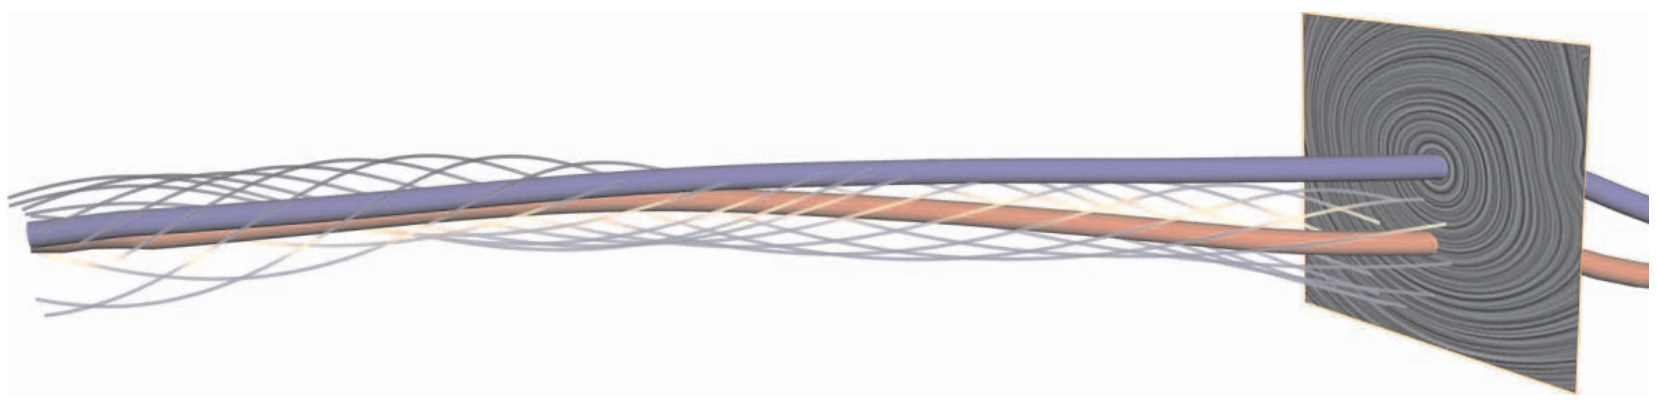
\includegraphics[width=\textwidth]{figures/pathline_streamline_core.png}
    \caption{Streamlines and pathlines swirl around different cores. The red
    tube shows the core of pathlines of a \ac{2D} vector field (rendered in
    \ac{3D} spacetime). The blue tube shows the path of the vortex core
    extracted from the individual time slices. Source: Weinkauf
    \etal~\cite{Weinkauf2007}.}
    \label{fig:cores_of_swirling_particle_motion}
\end{figure}
%
% subsubsection cores_of_swirling_particle_motion (end)
%
\subsubsection{Near-Steady Frame} % (fold)
\label{ssub:near_steady_frame}
%
The optimal reference frame for observing a vortex is a frame that follows the
vortex center over time~\cite{Robinson1991}.
%
In such a frame, the observed vector field around the vortex becomes almost
steady as ambient effects of larger flow structures are eliminated.
%
This is the basis of the approach proposed by G\"unther
\etal~\cite{Guenther2017}.
%
For each point in the flow, a locally optimal reference frame is computed in
which the flow becomes almost steady.
%
The reference frame is determined for a finite-sized neighborhood via a simple
linear optimization.
%
Once the vector field (and its derivatives) have been ``objectified'', any
region- or line-based vortex extractor that is designed for steady vector fields
can be used to extract objective unsteady vortices.
%
% subsubsection near_steady_frame (end)
%
% subsection vortices (end)
%
\subsection{Lagrangian Coherent Structures} % (fold)
\label{sub:lagrangian_coherent_structures}
%
\acf{LCS} are structures that show a locally maximal attracting or repelling
behavior of massless particles.
%
As the name suggests, these structures also tend to stay coherent over longer
time periods.
%
They can be thought of as a counterpart to vortices.
%
Whereas vortices represent the centers of swirling behavior, \ac{LCS} tend to
be located at the boundaries between vortices.
%
They act as transport barriers that have a minimal transverse flux of material
and are therefore very important for the investigation of mixing and transport
processes.
%
There are a number of very different methods for the investigation of \ac{LCS}.
%
A survey and comparison of some notable methods can be found
in~\cite{Hadjighasem2017}.
%

%
One popular approach to detecting \ac{LCS} is the investigation of the local
Lyapunov exponent~\cite{Ott2002}.
%
The Lyapunov exponent describes the rate of separation of infinitesimally close
trajectories over an infinite time interval.
%
Since real-world data is usually finite in time and space, two approximations of
the Lyapunov exponent are commonly used in practice: the
\emph{\acl{FTLE}\acused{FTLE}} (\acs{FTLE})~\cite{Haller2001} and
\emph{\acl{FSLE}\acused{FSLE}} (\acs{FSLE})~\cite{Aurell1997}.
%
It has been shown that ridges of the \ac{FTLE} or \ac{FSLE} field correspond
well to the locations of \ac{LCS}~\cite{Shadden2005,Haller2001}.
%

%
The basis for the computation of both \ac{FTLE} and \ac{FSLE} is the right
Cauchy-Green deformation tensor
%
\begin{equation*}
    \mC(\vx, t_0, t) = \T{\mF(\vx, t_0, t)}\, \mF(\vx, t_0, t) \,\text{,}
\end{equation*}
%
where $\mF$ is the deformation gradient obtained from the derivative of the
flow map
%
\begin{equation*}
    \mF(\vx, t_0, t) = \bPhi(\vx, t_0, t)\T{\nabla}\text{.}
\end{equation*}
%
The Cauchy-Green tensor describes the deformation the infinitesimal neighborhood
of a point $\vx$ at time $t_0$ experiences when advecting with the flow until
time $t$.
%
The maximum eigenvalue $\lambda_{\textnormal{max}}$ of this tensor is a measure for
the maximum separation of two particles starting in this infinitesimal
neighborhood.
%
\subsubsection{Finite-Time Lyapunov Exponent} % (fold)
\label{ssub:ftle}
%
The \acl{FTLE} measures the maximum separation of neighboring particles after
advecting with the flow for a finite time:
%
\begin{equation*}
    \text{FTLE}(\vx, t_0, \tau)
        = \frac{1}{|\tau|}
          \ln\sqrt{\lambda_{\max}\left[\mC(\vx, t_0, t_0 + \tau)\right]}\,\text{.}
\end{equation*}
%

%
A straightforward way of approximating the \ac{FTLE} of a flow is to compute the
flow map $\bPhi$ on a discrete grid and estimate the deformation gradient $\mF$
via central differences.
%
Since the ridges of an \ac{FTLE} field can become very sharp with increasing
time interval $\tau$, this is usually not very accurate.
%
Additionally, we are usually not interested in an accurate estimation of regions
without ridges.
%
For this reason, there are multiple numerical schemes for more precise or
performant \ac{FTLE} computations.
%
A good overview of the existing methods is provided in Alexander Kuhn's PhD
thesis~\cite{Kuhn2013}.
%
\begin{figure}[t]
    \centering
    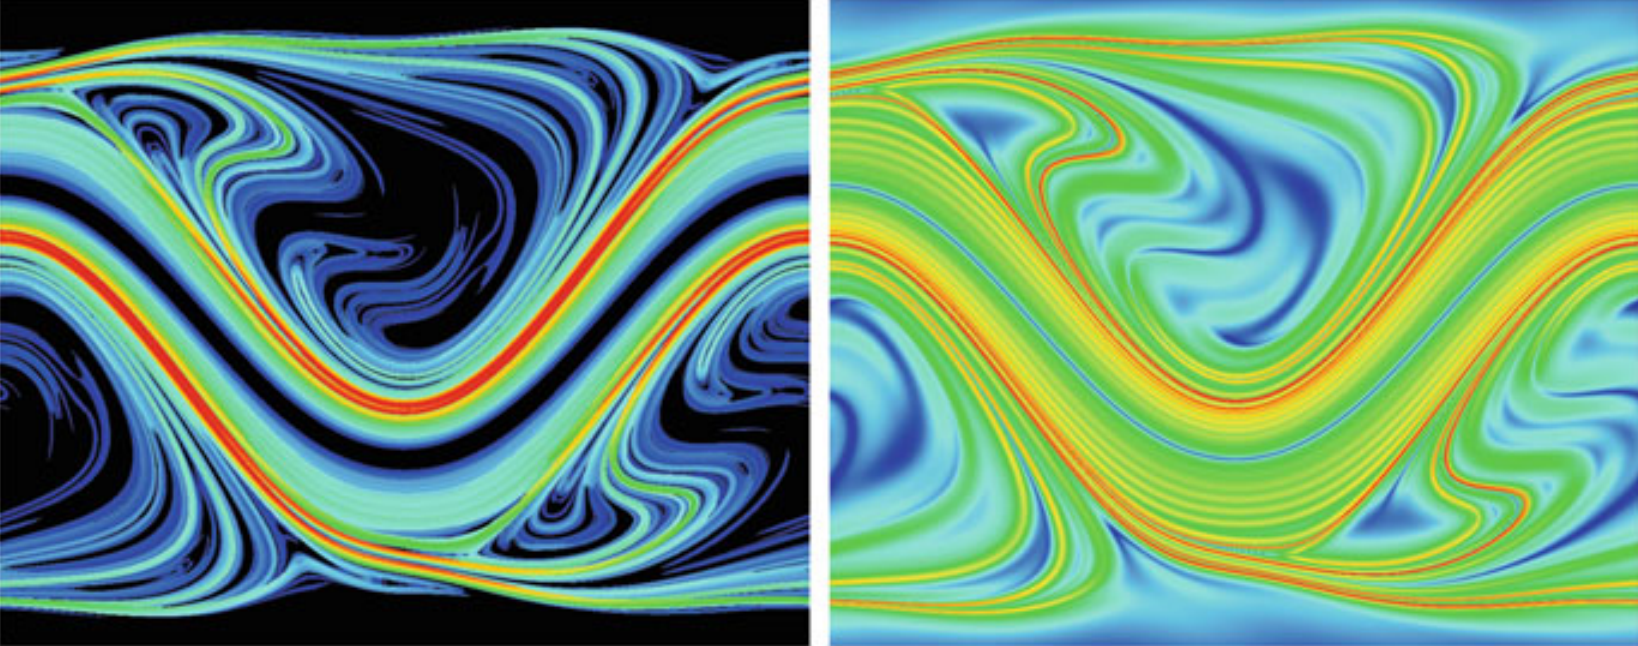
\includegraphics[width=\textwidth]{figures/fsle_ftle_peikert.png}
    \caption{Comparison of \ac{FSLE} (left) and \ac{FTLE} (right) of the flow
    field of a meandering jet. Image source: Peikert \etal~\cite{Peikert2014}.}
    \label{fig:ftle_fsle}
\end{figure}
%
% subsubsection ftle (end)
%
\subsubsection{Finite-Size Lyapunov Exponent} % (fold)
\label{ssub:fsle}
%
The \acl{FSLE} measures the time a pair of infinitesimally close particles
need to separate by a constant amount in space:
%
\begin{equation*}
    \text{FSLE}(\vx, t_0, r) = \frac{1}{|\tau_r|} \ln{r}\,\text{,}
\end{equation*}
%
where $\tau_r$ is the minimum time interval for which
%
\begin{equation*}
    \sqrt{\lambda_{\max}\left[\mC(\vx, t_0, t_0+\tau_r)\right]} = r\,\text{.}
\end{equation*}
%

%
\ac{FSLE} is popular in the oceanography community, but has not been adopted
much in the general visualization community.
%
As a result, \ac{FSLE} computation schemes in the literature are mostly
straightforward.
%
Either the maximum separation $\lambda_{\max}$ is estimated by a discrete
sampling of the flow map in different
directions~\cite{dOvidio2004,Hernandez-Carrasco2011}, or the Cauchy-Green tensor
is estimated based on central differences~\cite{Peikert2014}.
%

%
\ac{FTLE} and \ac{FSLE} yield similar results, given the right parameters (see
\cref{fig:ftle_fsle}).
%
However, their semantic differences might make one or the other more appropriate
depending on the application.
%
While \ac{FTLE} operates on a finite integration time $\tau$, which must be
estimated a-priori, it shows the behavior of the flow for all scales of spatial
separation.
%
In contrast, \ac{FSLE} needs the choice of a separation size, which might be
more intuitive.
%
It yields information about separation at different spatial scales, but it does
not show separation that is smaller than the given threshold $r$.
%
% subsubsection fsle (end)
%
% subsection lagrangian_coherent_structures (end)
%
% section vector_fields (end)